\section{Conntextualização}
\begin{frame}{Como vocês realizam as buscas por artigos?}
	\centering
	\begin{figure}
		
\includegraphics[width=1\textwidth]{figures/databases.jpg}
	\end{figure}
\end{frame}

\begin{frame}{Pouco tempo para muito resultado}
	\centering
	\begin{columns}
		\column{.5\textwidth}
				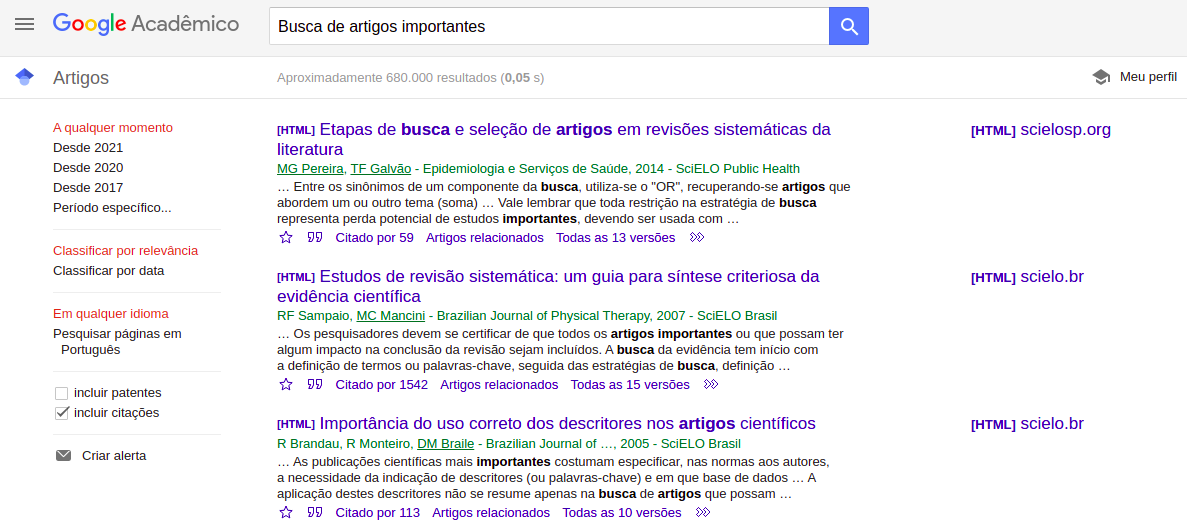
\includegraphics[width=1\textwidth]{figures/googleacademico2.png}
		\column{.5\textwidth}
				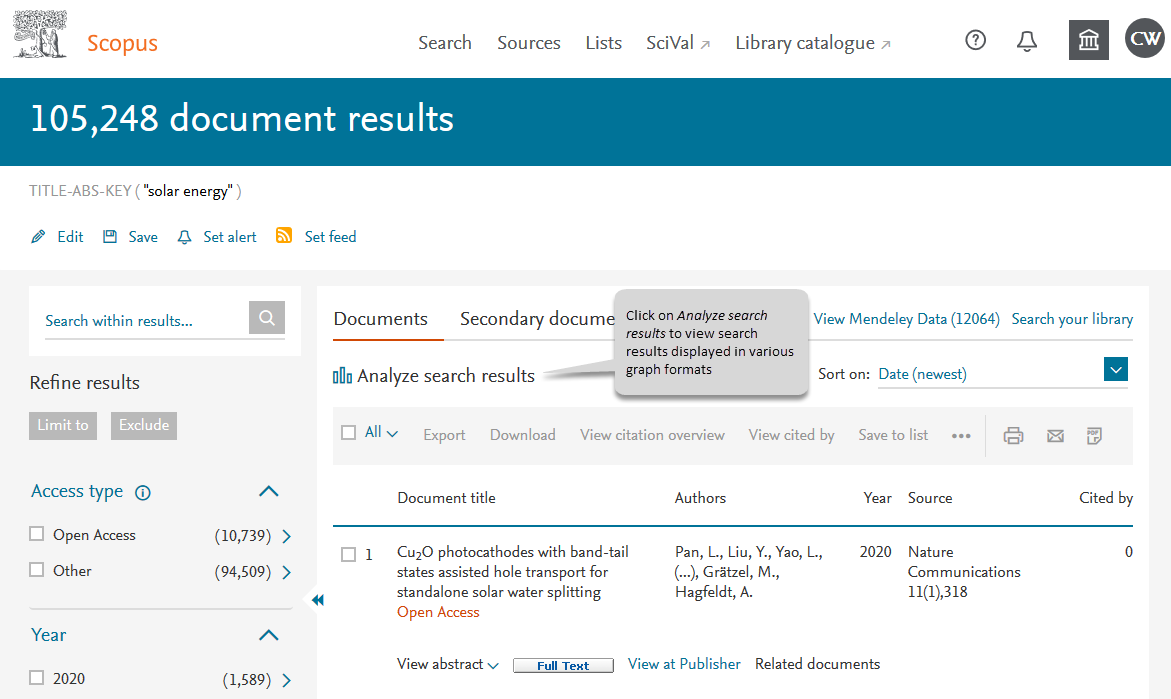
\includegraphics[width=1\textwidth]{figures/scopus.png}
	\end{columns}
	\begin{figure}
		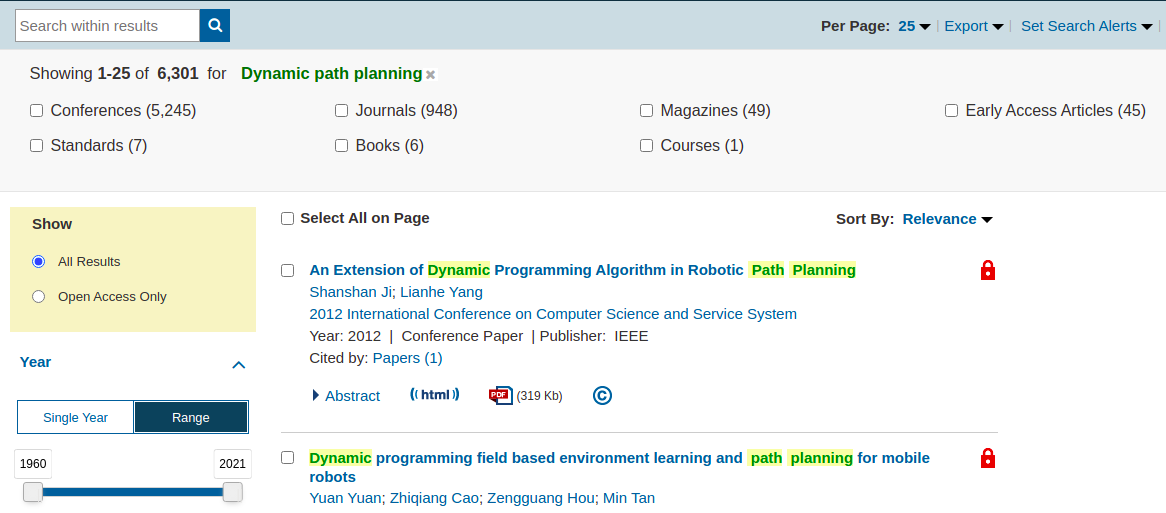
\includegraphics[width=.6\textwidth]{figures/ieee.png}	
	\end{figure}
\end{frame}

\begin{frame}{Tempo e precisão}
	A tecnologia existe para ajudar a nos tornar cada vez mais rápidos e precisos no que fazemos. 

	\begin{columns}
		\column{.5\textwidth}
		Fatores que impulsiona a ser rápido e preciso:
				\begin{itemize}
					\item Competitividade
					\item Prazo de entrega
					\item Concluir um trabalho 
				\end{itemize}
		\column{.5\textwidth}
		\begin{figure}[hb]
			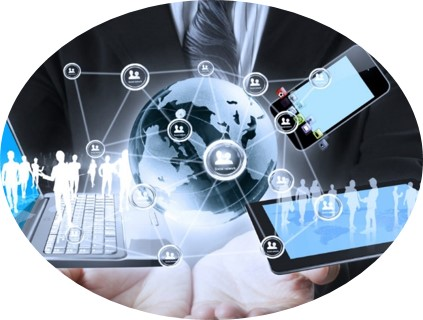
\includegraphics[width=1\textwidth]{figures/servicos.jpg}
		\end{figure}
	\end{columns}
\end{frame}

\begin{frame}{Existe algum método para melhorar a busca de artigos?}

	\begin{columns}
		\column{.3\textwidth}
		\begin{itemize}
			\item Biblioteconomia
			\item Método BiLi
		\end{itemize}
		\column{.8\textwidth}
		\begin{figure}[hb]
			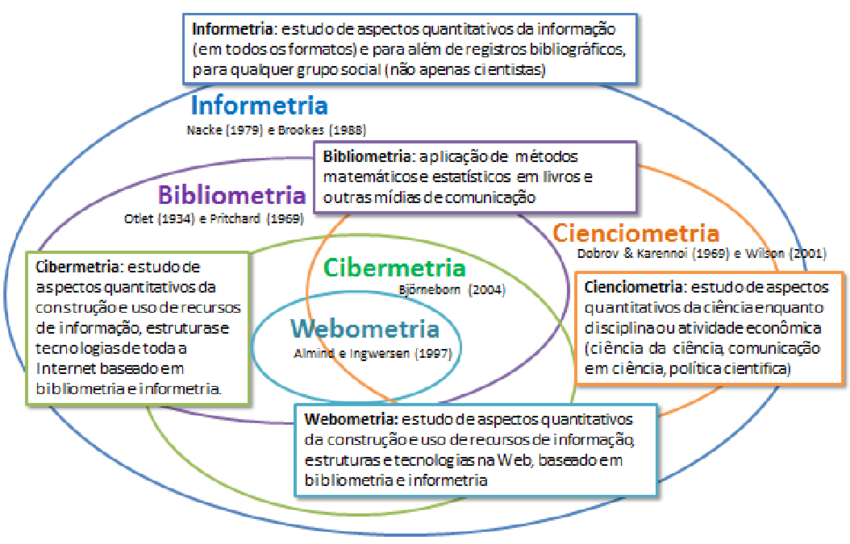
\includegraphics[width=1\textwidth]{figures/biblioeconomia.png}
		\end{figure}
	\end{columns}
\end{frame}

\begin{frame}{Bibliometria}
	\begin{columns}
		\column{.6\textwidth}
		\begin{itemize}
			\item Aplica métodos estatísticos e matemáticos para analisar e construir indicadores sobre a dinâmica e evolução da informação científica e tecnológica.
			\item Medir o desenvolvimento, a qualidade e o impacto de uma série de artigos escolhidos.
			\item Paul Otlet, 1934
		\end{itemize}
		\column{.4\textwidth}
		\begin{figure}[hb]
			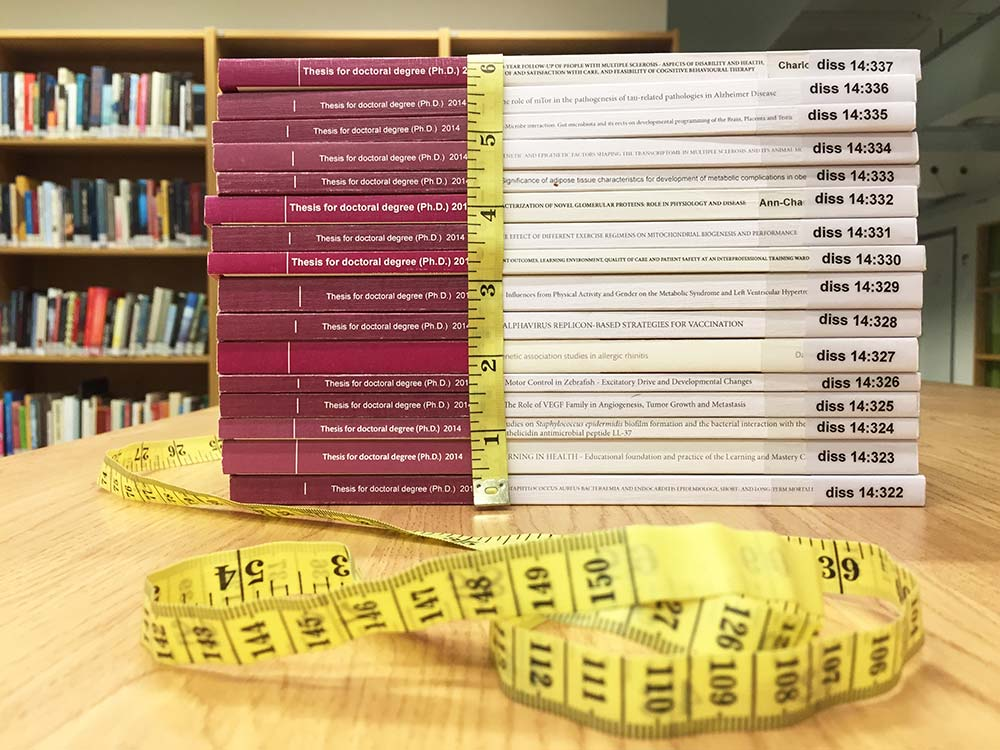
\includegraphics[width=1\textwidth]{figures/bibliometria.jpg}
		\end{figure}
	\end{columns}
\end{frame}

\begin{frame}{Três leis básicas}
	\begin{figure}[hb]
		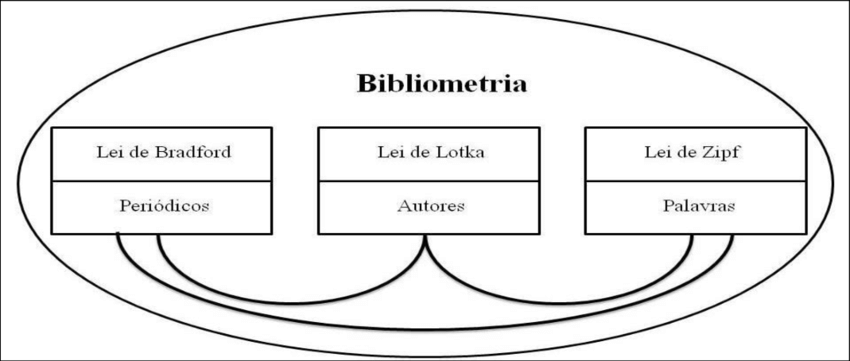
\includegraphics[width=1\textwidth]{figures/leisbibliometria.png}
	\end{figure}
\end{frame}

\begin{frame}{Lei de Bradford}

	\begin{columns}
		\column{.6\textwidth}
		Lei da dispersão
		\begin{itemize}
			\item Medir produtividade dos periódicos
			\item Estabelecer núcleo e as áreas de dispersão 
			\item Permite fazer a estimativa do grau de relevância das revistas de conhecimentos
		\end{itemize}
		\column{.4\textwidth}
		\begin{figure}[hb]
			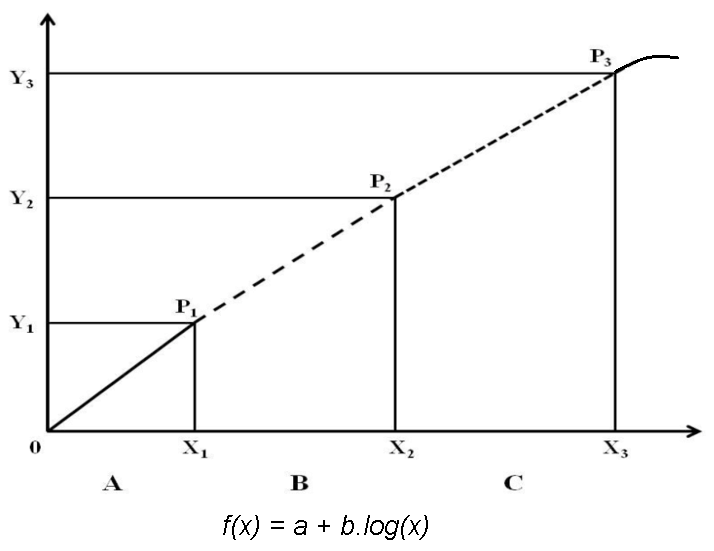
\includegraphics[width=1\textwidth]{figures/bradford.png}
		\end{figure}
	\end{columns}

\end{frame}

\begin{frame}{Lei de Lotka}

	\begin{columns}
		\column{.6\textwidth}
		Lei do quadrado inverso
		\begin{itemize}
			\item Produtividade dos autores	
			\item Relação entre o número de autores e o número de artigos publicados
			\item Alguns autores de maior prestígios produzem muito e muitos autores de menor prestígios produzem pouco
			\item Define as maiores contribuições dos pesquisadores
		\end{itemize}
		\column{.4\textwidth}
		\begin{figure}[hb]
			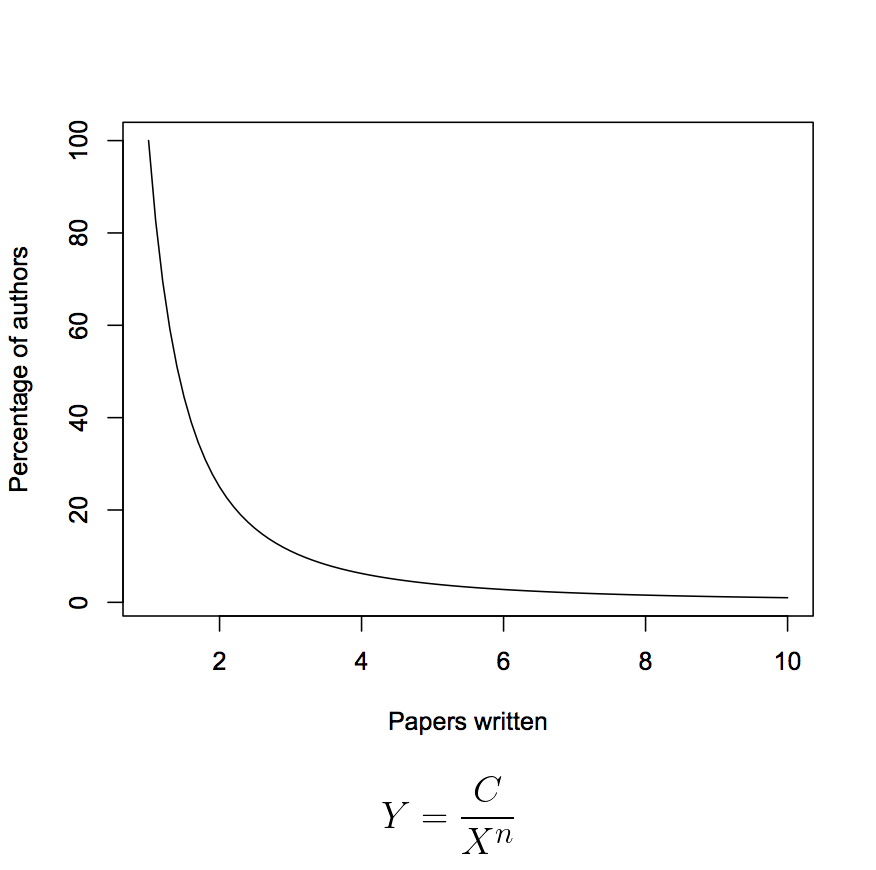
\includegraphics[width=1\textwidth]{figures/lokta.png}
		\end{figure}
	\end{columns}

\end{frame}

\begin{frame}{Lei de Zipf}

	\begin{columns}
		\column{.6\textwidth}
		Lei do menor esforço
		\begin{itemize}
			\item Trata e mede a frequência de ocorrência de palavras em vários textos
			\item As palavras mais usadas indicam o assunto
		\end{itemize}
		\column{.4\textwidth}
		\begin{figure}[hb]
			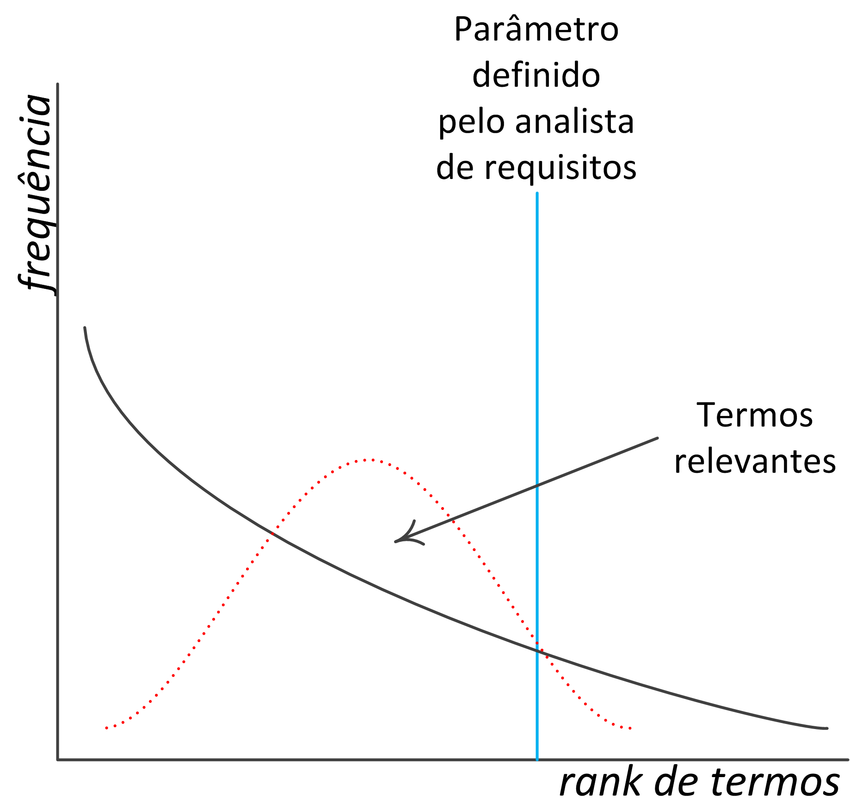
\includegraphics[width=1\textwidth]{figures/zipflunh.png}
		\end{figure}
	\end{columns}

\end{frame}

\begin{frame}{Fator de Impacto}

	\begin{columns}
		\column{.6\textwidth}
		Medida que reflete o número médio de citações de artigos científicos publicados.
		Avaliar a importância de um dado periódico em sua área.
		\column{.4\textwidth}
		\begin{figure}[hb]
			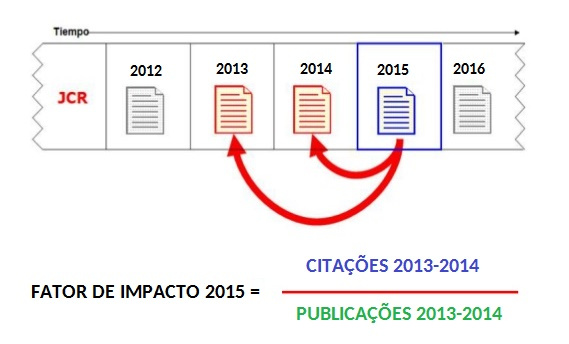
\includegraphics[width=1\textwidth]{figures/fi.jpg}
		\end{figure}
	\end{columns}

\end{frame}

\begin{frame}{Principais estudos da Bibliometria}

	\begin{table}[!h]
		\scalefont{0.7}
		\begin{tabular}{|l|c|l|}
		\hline
		\multicolumn{1}{|c|}{\textbf{Leis e Princípios}} & \textbf{Focos de Estudo} & \multicolumn{1}{c|}{\textbf{Principais Aplicações}}                                                                         \\ \hline
		Lei de Bradford                                  & periódicos               & \begin{tabular}[c]{@{}l@{}}estimar o grau de relevância de periódicos\end{tabular}         \\ \hline
		Lei de Lotka                                     & autores                  & \begin{tabular}[c]{@{}l@{}}estimar o grau de relevância de autores\end{tabular}            \\ \hline
		Leis de Zipf                                     & palavras                 & \begin{tabular}[c]{@{}l@{}}indexação automática de artigos científicos\\ e tecnológicos\end{tabular}                        \\ \hline
		Fator de Imediatismo ou de Impacto               & citações                 & \begin{tabular}[c]{@{}l@{}}estimar o grau de relevância de artigos, \\ cientistas e periódicos científicos\end{tabular} \\ \hline
		Acoplamento Bibliográfico                        & citações                 & \begin{tabular}[c]{@{}l@{}}estimar o grau de ligação de dois ou mais \\ artigos\end{tabular}                                \\ \hline
		Co-citação                                       & citações                 & \begin{tabular}[c]{@{}l@{}}estimar o grau de ligação de dois ou mais \\ artigos\end{tabular}                                \\ \hline
		Obsolescência da Literatura                      & citações                 & \begin{tabular}[c]{@{}l@{}}estimar o declínio da literatura de \\ determinada área do conhecimento\end{tabular}             \\ \hline
		Vida-média                                       & citações                 & \begin{tabular}[c]{@{}l@{}}estimar a vida-média de uma unidade da\\  literatura de dada área do conhecimento\end{tabular}   \\ \hline
		\end{tabular}
		\end{table}

\end{frame}